\chapter{Vierte Iteration - Übersichtlichkeit}
Die während der dritten Iteration in \autoref{chap:pro3} identifizierten Usability-Probleme und Anwenderwünsche sollen in diesem Kapitel weiter evaluiert werden.
Hierzu wird eine weitere Iteration des \hcdp{} ausgeführt.

\section{Observation}
Um die in \autoref{sec:test3} beschriebenen Probleme hinsichtlich ihrer Entstehung genauer zu untersuchen, werden diese zunächst aufgelistet und anschließend weiter beleuchtet.

\begin{itemize}
  \item Verwendung mehrerer Freitext-Formen im Bild zu unübersichtlich
  \item Doppelte Eingabe des Bildtitles beim Speichern irritierend
  \item Ungewollte Rotation von importieren Bildern
\end{itemize}

\noindent
Beide Testpersonen berichten in \autoref{sec:test3} von einer Unübersichtlichkeit bei der Verwendung von mehreren Text-Formen.
Dies hängt damit zusammen, dass die Schriftgröße des Textes dem aktuellen Zoom-Level der App angepasst wird.
So verkleinert sich der Text, wenn der Nutzer in das Bild hereinzoomt, und vergrößert sich wieder, sobald dieser herauszoomt.
Auf diese Weise soll sichergestellt werden, dass der Text unabhängig vom Zoom-Level jederzeit leicht lesbar ist.
Im herausgezoomten Zustand wird die Schriftgröße jedoch so stark vergrößert, dass die gesamte Freitext-Form zu viel Platz auf dem Bildschirm einnimmt.
Dies ist besonders auffällig, wenn der Nutzer mehrere Freitext-Formen erstellt, da diese anfangen sich zu überlappen und einen Großteil des Sichtbereiches zu verdecken.
(Nielsen~\autoref{itm:N12}) \\ 

Außerdem zeigen die Testergebnisse, dass es beim Speichern des bearbeiteten Bildes zu einer doppelten Eingabe des Titels kommt.
So muss der Benutzer einmal beim Speichern des Bildes innerhalb der \emph{Library} eine Beschreibung eingeben, und anschließend ein zweites Mal beim Hochladen des Bildes in der bestehenden App.
Diese doppelte Eingabe der exakt gleichen Beschreibung ist für den Benutzer nicht nachvollziehbar und sorgt darüber hinaus für unnötige Verwirrung.
(Nielsen~\autoref{itm:N1} \& \autoref{itm:N17}) \\

Zudem berichten beide Tester, dass sich im Hochformat aufgenommene Bilder ohne jegliche Interaktion beim Importieren in die App ins Querformat drehen.
Dieser Punkt ist beim lokalen Testen während der Implementierung des Prototyps auf keinem der benutzten Geräten aufgefallen.
Da beide Testpersonen ein \emph{Samsung}-Gerät verwenden, könnte es sich hierbei um einen Herstellerspezifischen Fehler handeln.
Auffällig ist auch, dass die beschriebene Rotation des Bildes nur dann geschieht, wenn das Bild beim Import weder skaliert noch zugeschnitten wurde.
Dieses Verhalten lässt sich im \emph{Quellcode} der \emph{uCrop-Library} verifizieren.
Hier wird vor dem Zuschneiden des Bildes geprüft, ob der Nutzer das Bild angepasst hat.
Ist dies nicht der Fall, so wird das Originalbild ohne jegliche Modifikation in die Zieldatei geschrieben.
Hierbei gehen auf \emph{Samsung}-Geräten die \emph{Exif}-Daten\urlnote{https://www.prophoto-online.de/digitalfotografie/exif-daten-10010057}{09.02.2018} verloren.
(Nielsen~\autoref{itm:N5}) \\ 

\section{Idea Generation}\label{sec:idea4}
Um das Bild auch bei der Verwendung von mehreren Freitext-Formen übersichtlich zu halten, bietet es sich an die Schriftgröße des Textes konfigurierbar zu machen.
Eine Alternative hierzu wäre es, die Formen aufklappbar zu gestalten, sodass der Nutzer selber entscheiden kann, welche Notiz zu welcher Zeit sichtbar sein soll, und welche zum Beispiel nur als \emph{Icon} auf dem Bild zu sehen ist. \\

Die doppelte Eingabe der Bildbeschreibung beim Speichern lässt sich durch das Einführen eines weiteren Parameters beim Starten der Library lösen.
So kann beim Benutzen der \emph{Library} über den zusätzliche Parameter entschieden werden, ob beim Speichern ein Speicher-Dialog innerhalb der \emph{Library} angezeigt werden soll oder nicht.
Hierdurch lässt sich der Speicher-Dialog für die bestehende App einfach ausblenden, und das doppelte Eintragen des Bildtitels verhindern. \\

Das ungewollte Rotieren von Bilder, die im Hochformat aufgenommen wurde, kann durch eine spezielle Überprüfung des Geräteherstellers verhindert werden.
Diese Überprüfung soll das Bild, wenn es sich um ein Geräte von \emph{Samsung} handelt, auch dann zuschneiden, wenn der Nutzer keine Modifikation am Bild vorgenommen hat.
Hierdurch soll sichergestellt werden, dass die \emph{Exif}-Daten nicht verloren gehen und das Bild nicht ungewollt rotiert wird.

\section{Prototyping}
Der vierte Prototyp wurde am 10. Februar 2018 ausgerollt und in die bestehende Android-App eingebunden, um die in \autoref{sec:idea4} genannten Lösungsideen umzusetzen. \\

Für eine bessere Übersichtlichkeit bei der Verwendung von mehreren Freitext-Formen gleichzeitig, wurde die Funktion hinzugefügt, dass Freitext-Formen über einen Doppelklick ein- bzw. aufgeklappt werden könne.
So werden diese im ``ausgeklappten'' Modus wie zuvor als Text mit Hintergrund angezeigt, beim Doppelklick transformiert sich diese Form jedoch zu einem kleinen Icon, welches keinerlei Text anzeigt, und so nur suggeriert , dass sich hinter dem Icon eine Freitext-Form befindet. 
Dies soll dem Benutzer die Möglichkeit geben, selber zu entscheiden, welcher Text wann auf dem Bildschirm sichtbar ist und welcher nicht. \\

\begin{figure}[h]
  \begin{subfigure}[t]{0.4\textwidth}
    \centering
    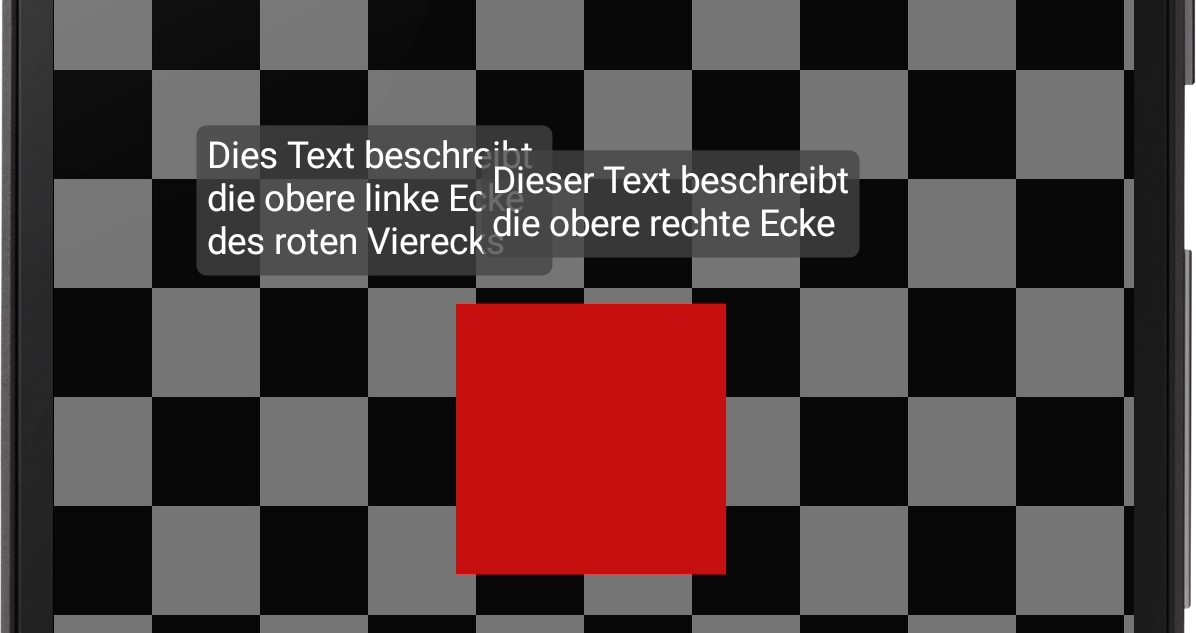
\includegraphics[keepaspectratio, width=\textwidth]{prototype4/text1}
    \caption{Zwei Freitext-Formen im dritten Prototyp}
  \end{subfigure}
  ~
  \begin{subfigure}[t]{0.4\textwidth}
    \centering
    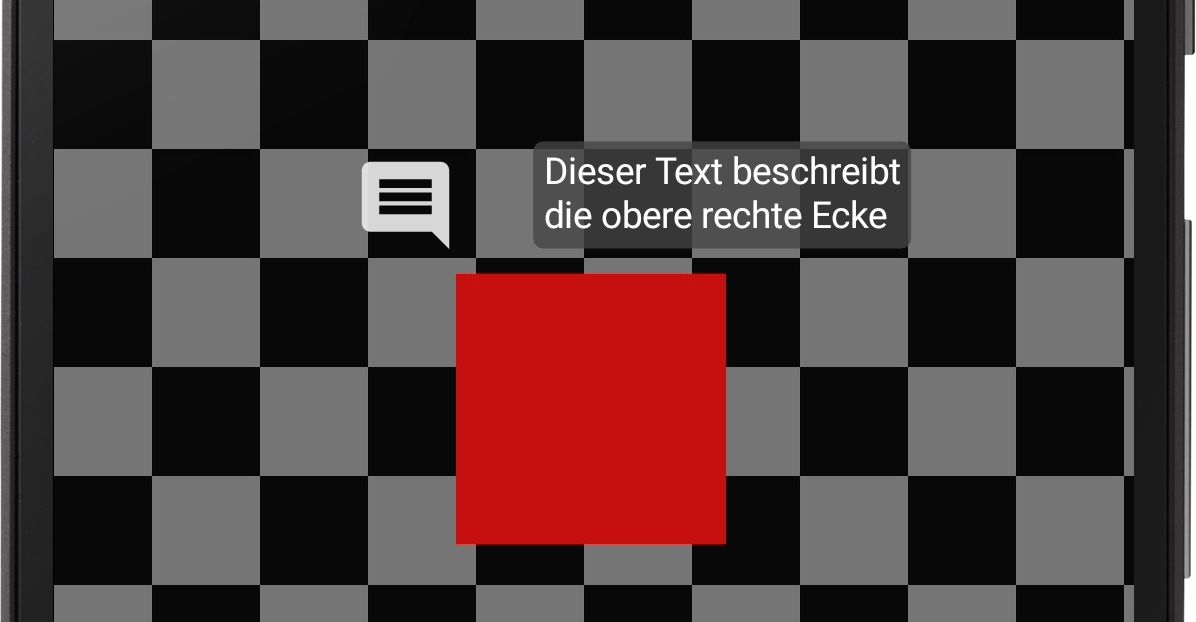
\includegraphics[keepaspectratio, width=\textwidth]{prototype4/text2}
    \caption{Zwei Freitext-Formen im vierten Prototyp (eine minimiert)}
  \end{subfigure}
  \centering
  \caption{Vorher-Nachher-Vergleich: Anzeige zweier Freitext-Formen im dritten und vierten Prototyp}
  \label{fig:texts}
\end{figure}

Der Speicher-Dialog wurde durch das Hinzufügen eines weiteren Start-Parameters in der \emph{Library} ausgeblendet, und ist so bei der Benutzung in der bestehenden Android-App nicht mehr zu sehen.
Hier wird das Bild direkt auf dem Gerät gespeichert und anschließend in der bestehenden App nach einem Bildtitel gefragt. \\

Die ungewollte Rotation der Bilder auf \emph{Samsung}-Geräten wurde durch die Modifikation der \emph{uCrop-Library} umgesetzt.
Hierzu wurde ein \emph{Fork}\urlnote{https://help.github.com/articles/fork-a-repo/}{10.02.2018} der \emph{Library} erstellt und anschließend eine Überprüfung des Geräteherstellers im \emph{Quellcode} hinzugefügt.

\section{Testing}
Feedback zum Benutzererlebnis des vierten Prototyps gab es 7 Tage nach dem Roll-Out, am 17. Februar. \\

In dieser vierten Iteration des \hcdp{} sind keine weiteren Usability-Probleme identifiziert worden.
Der Prototyp ließe sich, so beide Testpersonen, intuitiv und einfach zum Erfassen der Aufmaße verwenden und würde auf langer Sicht viel Arbeit und Zeit sparen, da alle Informationen sofort digital und für alle Mitarbeiter zur Verfügung stehen. \\

Ein abschließender Anwenderwunsch bezieht sich auf das  Herunterladen bereits annotierter Bilder zum Bearbeiten auf einem anderen Gerät.
Da dieser Anwenderwunsch von der Android-App alleine nicht umgesetzt werden kann, wurde eine solche Funktionalität von der bestehenden \emph{API} am 17. Februar angefordert.
Genauer soll hier ein weiterer Endpunkt auf Seiten der \emph{API} definiert werden, welcher die hochgeladenen Meta-Daten des bearbeiteten Bildes formatiert als \emph{JSON}\urlnote{https://www.json.org/json-de.html}{10.02.2018} entgegennimmt.
Zusätzlich soll ein Endpunkt zum Bereitstellen des annotierten Bildes inklusive Meta-Daten implementiert werden. 
Auf diese Weise soll es dem Benutzer möglich sein, annotierte Bilder zu einem späteren Zeitpunkt auf dem gleichen oder einem anderen Gerät bearbeiten zu können.
